% $File: report.tex
% $Date: Sat Nov 16 21:00:12 2013 +0800
% $Author: wyx <ppwwyyxxc@gmail.com>

\documentclass[11pt,a4paper]{article}
\usepackage{threeparttable}
\usepackage{dirtree}
\usepackage{keystroke}


\usepackage{fontspec,amsmath,amssymb,zhspacing,verbatim,minted,listings,zhmath}
\usepackage{titlesec, titletoc}
\usepackage{pdfpages}
\usepackage{enumerate}
\usepackage[hyperfootnotes=false,colorlinks,linkcolor=blue,anchorcolor=blue,citecolor=blue]{hyperref}
\usepackage[backend=biber]{biblatex}
%\usepackage[dvips]{graphicx}
\usepackage{subfigure}
\usepackage{indentfirst}
\usepackage{float}			% don't automatically change location of figure [H]
\usepackage{chngpage}		% use \changetext to change page size
\usepackage{caption}\captionsetup{hypcap=true}  % ref to jump to object instead of caption
\newfontfamily\zhfont[BoldFont=SimHei,ItalicFont=KaiTi_GB2312]{SimSun}
\lstset{keywordstyle=\color{blue!70}, commentstyle=\color{red!50!green!50!blue!50},frame=shadowbox,rulesepcolor=\color{red!20!green!20!blue!20},
basicstyle=\footnotesize\ttfamily}
\zhspacing
\setlength{\parindent}{2em}

\usepackage{fancyhdr}
\changetext{}{2.2cm}{-1.1cm}{-1.1cm}{}
\pagestyle{fancy}
\setlength{\headheight}{15.2pt}
\lhead[]{}\rhead[]{}
\fancyhead[C]{\emph{Design Document - Uknow InfoHub}}


%use cell in tabular
\newcommand{\tabincell}[2]{\begin{tabular}{@{}#1@{}}#2\end{tabular}}

%thick shline
\newlength\savewidth
\newcommand\shline{\noalign{\global\savewidth\arrayrulewidth\global\arrayrulewidth 1pt}
                   \hline
                   \noalign{\global\arrayrulewidth\savewidth}}


\defbibheading{bibliography}{\section{References}}
\bibliography{refs.bib}
\newcommand{\figref}[1]{\hyperref[fig:#1]{Fig. \ref*{fig:#1}}}
\newcommand{\secref}[1]{\hyperref[sec:#1]{Sec. \ref*{sec:#1}}}
\newcommand{\tabref}[1]{\hyperref[tab:#1]{Tab. \ref*{tab:#1}}}

% math function
\let\Oldsum\sum
\renewcommand{\sum}{\displaystyle\Oldsum}
\let\Oldprod\prod
\renewcommand{\prod}{\displaystyle\Oldprod}


../mint-defs.tex

\title{Uknow InfoHub \\ \small Design Document}
\author{BlXLRSMB Team}
\date{}

\begin{document}

\titleformat*{\section}{\centering\Large\bf}
\titleformat*{\subsubsection}{\large\bf}
\setlength{\baselineskip}{1.3em}
\fontsize{12}{\baselineskip}\selectfont


%
\includepdf{img/cover}
\maketitle
\tableofcontents
\newcolumntype{L}{>{\centering\arraybackslash}m{3cm}}

\section{Introduction}
\label{sec:intro}
\subsection{Document Introduction}
\label{sec:introduction}
	In the following sections of this document, we will present several skim of our project management.

	In~\secref{git}, how we use git as the subversion tool. Issues and milestones will be presented in~\secref{issue}.



\section{Architecture}
%File: functional-user.tex
%Date: Sat Oct 19 17:05:21 2013 +0800
%Author: Yikai Zhao <blahgeek@gmail.com>

\subsection{Fetcher}
  As the core component, fetcher is designed to be extremely flexible.
  It will be inherited into various kinds of fetchers to deal with different fetch target.
  All the fetchers will be executed in a cluster as a time based work, just like web spiders, keeps fetching all the time.
  \begin{figure}[H]
    \centering
    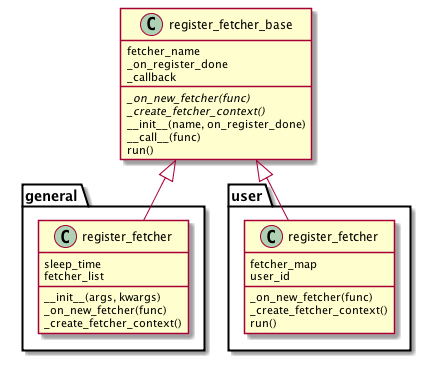
\includegraphics[width=0.6\textwidth]{img/fetcher.png}
    \caption{Fetcher\label{fig:fetcher}}
  \end{figure}

  \subsubsection{Function}
    The fetcher will be assigned to a target website or other kind of source.
    Each time it was called, it will return a list of informations, almost in raw text but with some basic information,
    such as source, origin url, fetched time and so on.

  \subsubsection{Performance}
    Fetcher shall be called at least one time per day. For hot resources such as SNS, it's fetcher must have high speed,
    so each time it shall return result in minute level.

  \subsubsection{Input}
    Fetcher don't need input after it's well configured. However, for augmentbility reason, a callback function is acceptable.
    The callback funtion will deal with the result by default.

  \subsubsection{Output}
    Fetcher will return a FetcherContext which wraps the raw information. For default situation, it will be dealed by Prefilter.


%File: functional-user.tex
%Date: Sat Oct 19 17:05:21 2013 +0800
%Author: Yikai Zhao <blahgeek@gmail.com>

\subsection{Prefilter}
  What users want definitely is not raw information. Thus a prefilter will be applied on each piece of information after it's fetched.
  Prefilter will be called each time a fetcher returned a piece of information, then if it's not abandoned, prefilter will save it into database.

  \begin{figure}[H]
    \centering
    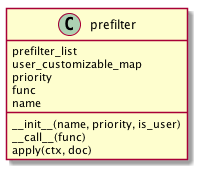
\includegraphics[width=0.4\textwidth]{img/prefilter.png}
    \caption{Prefilter\label{fig:prefilter}}
  \end{figure}

  \subsubsection{Function}
    Prefilter is the first classifier applied on the information. It can be system defined or user customized.
    Itself has priority levels, thus different prefilter will be executed on a information in order.
    It will put different tags on a piece of information, so in the next step it can be selected out easily.

  \subsubsection{Performance}
    It shall give the result almost immediately after it was called. So it only has several seconds of time.

  \subsubsection{Input}
    A FetcherContext item which was just fetched by a fetcher.

  \subsubsection{Output}
    A FetcherContext item which has multiple tags base on its content read by prefilter.
    Notice that a item may be abandoned by a prefilter for it may be duplicate, redundant or illegal.


%File: functional-user.tex
%Date: Sat Oct 19 17:05:21 2013 +0800
%Author: Yikai Zhao <blahgeek@gmail.com>

\subsection{Postfilter}
  Users can't read all of information that we fetched.
  Thus a postfilter is designed to search for information that users want to read.
  It will be called each time user make a action that need get new information.

  \subsubsection{Function}
    Postfilter is designed aimed to select the best information that users want.
    It will pick out information that have the same or similiar tags with what user request.
    More, it will sort the information list in better order so user can get what they are most desired to get at first skim.

  \subsubsection{Performance}
    For that users must wait for it when ask for more information, it shall have extremely high Performance, as fast as possible.

  \subsubsection{Input}
    A user defined query request, has various properties and limits.

  \subsubsection{Output}
    A list of information, which fits users request well.


%File: functional-user.tex
%Date: Sat Oct 19 17:05:21 2013 +0800
%Author: Yikai Zhao <blahgeek@gmail.com>

\subsection{API Website}
  All things talking above is though as the backend and core items of this project.
  What exposed to client software is the api website. Which will run in Linode server so that every client can find it easily.

  \subsection{Function}
    API website will check the requester's permission and validate the request format.
    Then it will call the components described above to get the response, then provide them to the requester.

  \subsection{Performance}
    The same, users must wait for it when posting request, it shall have extremely high performance.

  \subsection{Input}
    Various kinds of request.

  \subsection{Output}
    Responses to them.



\section{Data Storage}
  \subsection{Session}
    Session that used to determine which user is currently posting request is stored in redis which is a light key-value pair database.
    Though only one value can be stored in one key, its high performance makes it's the best to store sessions data.

    The sessions is stored automatically without any design, for a third party package will handle all of this.

  \subsection{Item}
    Item mainly is the only things that we need to store other than user's information which needed for all apps.

    With considering of that each piece of information mainly doesn't have relationship with others but has multiple complex attributes in itself,
    NoSQL that doesn't need table structure but store data in documents is what we want.

    An item will be mapped into a FetcherContext object in program, and it will be stored into database simply with all attributes
    in key-value pair format.

    \begin{figure}[H]
      \centering
      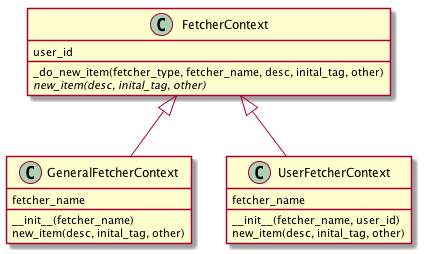
\includegraphics[width=0.6\textwidth]{img/fetcherContext.png}
      \caption{FetcherContext\label{fig:fetcherContext}}
    \end{figure}

  \subsection{Labels}
    Labels is a quite simple one in storage step.
    Each label is just a basic string describing itself. So it doesn't have even an individual table.
    Labels are stored as a part of Item, in a list as a sub node of it.

    For performance reason, Labels are often used to filtering out Items, so index was build according to it.


%
\includepdf{img/cover-normal}

\printbibliography

\end{document}

